\documentclass[a4paper, 12pt]{article}
\usepackage[utf8]{inputenc}
\usepackage[spanish]{babel}
\usepackage{url, hyperref}
\usepackage{graphicx}

\setlength{\parindent}{0pt}

\title{\vspace{-3cm}Examen Parcial 2: Vida Soldada con GA}
\author{
    Universidad Autónoma de San Luis Potosí\\
    Facultad de Ingeniería - Ing. en Sistemas Inteligentes\\
    \textbf{Materia:} Cómputo Bioinspirado\\
    \textbf{Autor:} Angel de Jesús Maldonado Juárez
}
\date{\textbf{Fecha de entrega:} martes 1 de noviembre de 2022}

\begin{document}
\maketitle

\hrule

\section{Planteamiento del problema}
En la construcción del edificio T de la Facultad de Ingeniería de la UASLP, la unión entre vigas de acero se hizo mediante el uso de tornillos. En la actualidad, se ha demostrado que una forma de economizar recursos en una construcción es utilizar soldadura en lugar de tornillos. Pero para que resulte realmente económico, es necesario hacer un balance entre la cantidad de soldadura utilizada y el peso que la viga está destinada a sostener.

La Figura \ref{fig:1} muestra el modelo gráfico de este problema. Se puede apreciar una viga soldada en el sustrato (el bloque mayor). La viga soporta una carga $P$ a una distancia $L$ del sustrato. La viga está soldada en la parte de arriba y abajo contra el sustrato (zona sombreada). Cada soldadura tiene una longitud $l$ y un grosor $h$. El peso de la viga se puede aproximar conociendo el ancho $b$ y la altura $t$ de la misma. Para simplificar el problema, la carga se define con un valor fijo de $P=6000lbs$; y la distancia del sustrato como $L=14in$.

Por lo tanto, las variables del problema son las siguientes: $h=x(1)=x_1$, $l=x(2)=x_2$, $t=x(3)=x_3$, $b=x(4)=x_4$.

\begin{figure}[!ht]
    \centering
    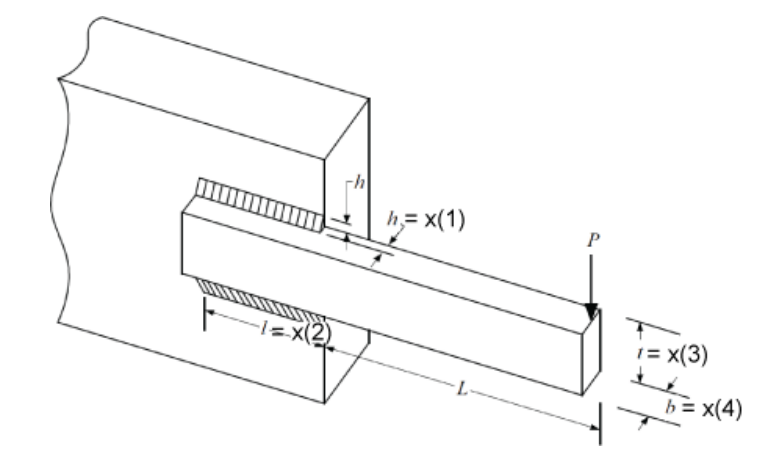
\includegraphics[width=0.4\textwidth]{img/modelo_problema.png}
    \caption{Modelo del problema \emph{Viga Soldada}.}
    \label{fig:1}
\end{figure}

La función que se va a \textbf{minimizar} ($F_w(x)$) es el \textbf{costo} de colocar la viga como se muestra en la Figura \ref{fig:1}, y se puede definir de la siguiente manera:

\begin{equation}
    F_w(x)=1.10471x^2_1x_2+0.04811x_3x_4(14+x_2)
\end{equation}

Minimizar esta función está sujeto a estas cinco restricciones:

\begin{enumerate}
    \item El grosor de la soldadura no debe ser mayor al ancho de la viga: $x_1\leq x_4$.
    \item La tensión diagonal $T$ que soporta la viga no puede ser mayor de $13600psi$: $13600\geq T$.

          \emph{Para calcular $T$, primero, se deben aplicar las siguientes fórmulas:}

          \begin{equation}
              \tau_1=\frac{1}{\sqrt{2}x_1x_2}
          \end{equation}

          \begin{equation}
              R=\sqrt{x_2^2+(x_1+x_3)^2}
          \end{equation}

          \begin{equation}
              \tau_2=\frac{(L + x_2/2)R}{\sqrt{2}x_1x_3(x_2^2/3+(x_1+x_3)^2)}
          \end{equation}

          \begin{equation}
              T(x)=P\sqrt{\tau_1^2+\tau_2^2+\frac{2\tau_1\tau_2x_2}{R}}
          \end{equation}

    \item La tensión $\sigma$ normal que soporta la viga no debe ser mayor a $30000psi$: $30000\geq\sigma$. Donde $\sigma=P\frac{6L}{x_4x_3^2}$.

    \item La capacidad de la viga antes de doblarse (capacidad de carga de pandeo, o $P_c$) debe ser mayor a la carga de $6000lbs$: $P_c\geq 6000$. Donde $P_c=64746.022(1-0.02822346x_3)x_3x_4^3$.

    \item El factor de peso $\delta$ no debe ser mayor a $0.25$: $0.25\geq \delta$. Donde $\delta=(2.1952/(x_3^3x_4))$.
\end{enumerate}

Se debe minimizar la función $F_w$ y convertir las restricciones que se mencionan, de manera que se puedan representar en los parámetros en un \emph{Algoritmo Genético} GA.

Una vez codificado el problema a minimizar con las restricciones, se debe ejecutar el algoritmo genético para obtener resultados lo más cercanos a los siguientes valores:

\begin{itemize}
    \item $F_w=2.38116$
    \item $x_1=0.2444$
    \item $x_2=6.2187$
    \item $x_3=8.2915$
    \item $x_4=0.2444$
\end{itemize}

\section{Descripción de la solución}

\section{Descripción de los resultados}

\section{Discusión}

\section{Conclusión}

\bibliographystyle{unsrt}
\bibliography{refs}
\nocite{*}
\end{document}